\section{Semaine 26 (05/05 - 09/05) }


\e{Notions abordées :}
\begin{itemize}
	\item Diagrammes E-pH (cf semaine précédente).
	\item Mécanique du solide.
\end{itemize}

\subsection{Questions de cours}

\begin{enumerate}
	\item Théorème de la résultante dynamique.
	\item Théorème du moment cinétique pour un solide en rotation autour d'un axe fixe.
	\item Théorème de la puissance cinétique pour un solide en rotation autour d'un axe fixe.
\end{enumerate}


\subsection{Exercice 1 : Chute d'une personne sur un poteau}

On considère un poteau vertical modélisé par une tige homogène rigide de masse $M$ et de longueur $L$. En $t=0$, un coup de vent déséquilibre le poteau et il commence à tomber, son extrémité basse restant en contact avec le sol. Soit $\Delta = (Oy)$ l'axe de rotation du poteau. Le moment d'inertie du poteau par rapport à $\Delta$ est $J_{\Delta} = \frac{1}{3}ML^2$. On repère sa position au cours du temps par l'angle $\theta$ par rapport à la verticale. 

Sur le poteau, une personne de masse $m$ est debout. On considère $m \ll M$ et on néglige donc le moment de la réaction de la personne sur le poteau dans l'étude du mouvement de ce dernier. 

\begin{enumerate}
	\item Déterminer l'équation du mouvement du poteau au cours de la chute.
	\item Intégrer cette équation et utiliser les conditions initiales pour déterminer $\dot{\theta}^2$ en fonction des données du problème et de $\theta$.
	\item À quelle condition la personne décolle-t-elle du poteau ?
	\item Exprimer la réaction normale du poteau sur la personne en fonction des données du problème, de $\dot{\theta}$ et de $\theta$.
	\item Déterminer l'angle auquel a lieu le décollage.
\end{enumerate}

\e{Réponse :} $\theta_{dec} = \arccos{\frac{3}{4}}$.

\subsection{Exercice 2 : Chute d'une tartine beurrée}

On modélise une tartine beurrée de masse $m$ par un parallélépipède rectangle de centre de gravité $G$. La tartine étant initialement posée au bord d'une table, elle se met à pivoter autour de l'axe fixe du bord de la table, axe que l'on note $(Iz)$. Soit $J = J_{(Iz)}$ le moment d'inertie de la tartine par rapport à cet axe. On repère le mouvement de la tartine par l'angle $\theta$ qu'elle fait par rapport à l'horizontale.

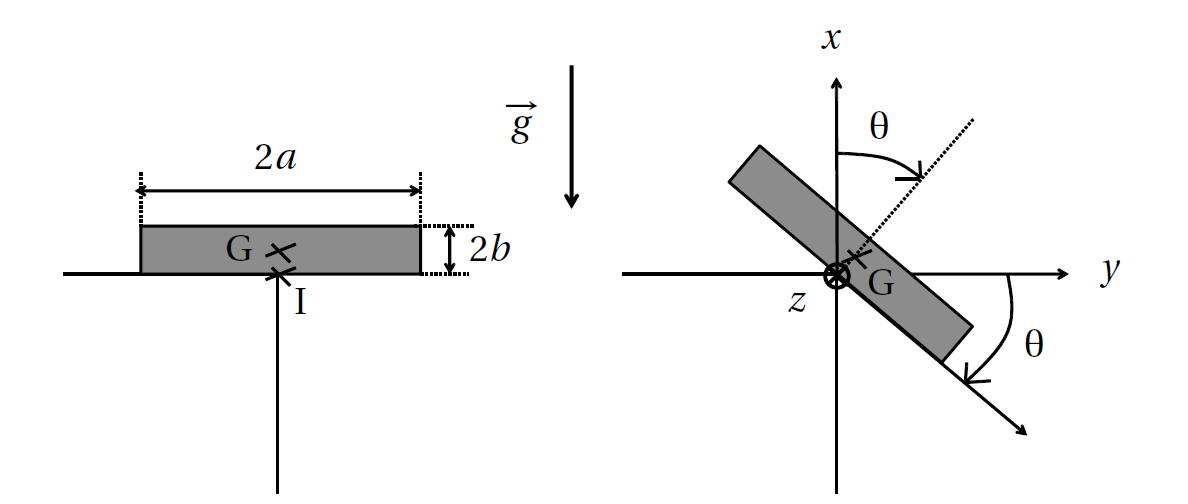
\includegraphics[width=\textwidth]{Images/mpsi_s26_ex02.png}

\begin{enumerate}
	\item Déterminer l'équation différentielle en $\theta$ qui régit le mouvement de rotation de la tartine.
	\item Par intégration, déduire l'expression de $\dot{\theta}$ en fonction des données du problème et de $\theta$.
	\item Quand $\theta = \pi/4$, la tartine commence à glisser et tombe de la table. Elle se retrouve alors en chute libre et on peut montrer qu'elle conserve la vitesse de rotation $\omega_0$ qu'elle avait en quittant la table. En déduire l'expression de $\omega_0$ et celle de $\theta(t)$ en fonction de $\omega_0$. On négligera le temps de glissement en considérant que le mouvement de chute libre commence avec $\theta(0) = \pi/4$, en prenant comme nouvelle origine des temps cet instant.
	\item En considérant approximativement que le temps de chute $t_c$ de la tartine est donné par le temps mis par $G$ pour atteindre le sol après une chute libre d'une hauteur $h$ et une vitesse initiale négligeable, exprimer $t_c$ en fonction de $g$ et $h$.
	\item On donne $J = \frac{1}{3}ma^2 + \frac{4}{3}mb^2$. On prend $g = \SI{9.8}{\meter\per\second\squared}$, $b = \SI{0.50}{\centi\meter}$, $a = \SI{8.0}{\centi\meter}$ et $h = \SI{0.80}{\meter}$. Déterminer numériquement $\omega_0$ et $t_c$. On pourra au préalable simplifier l'expression de $J$ au vu des valeurs de $a$ et $b$.
	\item En déduire numériquement $\theta(t_c)$. Commenter.
\end{enumerate}

\e{Réponses :}
\begin{enumerate}
	\item -
	\item $\dot{\theta} = \sqrt{\frac{2mgb(1-\cos\theta)}{J}}$
	\item $\omega_0 = \sqrt{\frac{mgb(2-\sqrt{2})}{J}}$
	\item -
	\item $\omega_0 = \SI{3.7}{\radian\per\second}$ et $t_c = \SI{0.40}{\second}$.
	\item $\theta(t_c) = \SI{132}{\degree}$
\end{enumerate}

\subsection{Exercice 3 : Suspension d'un tableau}

On suspend un tableau de masse $M$ de forme rectangulaire (largeur $a$ et hauteur $b$) au milieu $O$ d'un de ses côtés. Il peut osciller autour de l'axe $\Delta$ perpendiculaire au mur et passant par $O$. Le moment d'inertie du tableau par rapport à $\Delta$ est $J = \frac{M(a^2 + 4 b^2)}{12}$. En notant $G$ le centre de gravité, on repère la position du tableau par l'angle $\theta$ entre $\overrightarrow{OG}$ et la verticale passant par $O$.

\begin{center}
	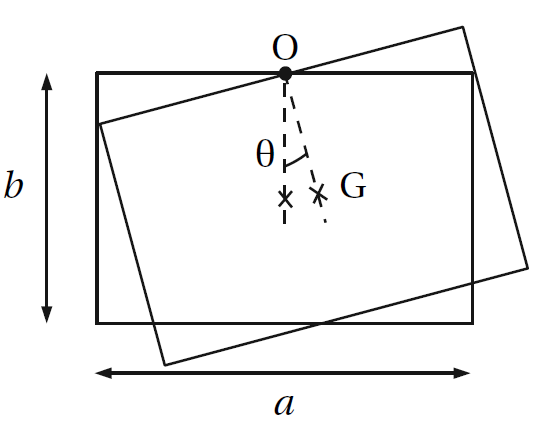
\includegraphics[width=.5\textwidth]{Images/mpsi_s26_ex03.png}
\end{center}

\begin{enumerate}
	\item Établir l'équation du mouvement des oscillations du tableau autour de $O$.
	\item On se place dans le cas des petites oscillations. Donner l'expression de la période de ces oscillations en fonction de $a$, $b$, et $g$.
	\item En supposant que la surface du tableau ne varie pas, comment varie la période des oscillations si on augmente la valeur de $a$ ?
	\item Même question si on augmente $b$.
\end{enumerate}
